\section{Problem Statement: Bipedal Walker Robot Control}
\label{sec:problem_statement}
\subsection{OpenAI Gym and Bipedal-Walker Environment}
\label{gym_bipedal}
OpenAI Gym \cite{brockman_openai_2016} is open source framework, containing many environments to service reinforcement learning algorithms. \\
Bipedal-Walker environments \cite{noauthor_bipedalwalker-v2_2021} \cite{noauthor_bipedalwalkerhardcore-v2_2021} is part of Gym environment library. One of them is classical version where the terrain is relatively smooth, while other one is hardcore version which contains ladders, stumps and pitfalls in terrain. \\
For both settings, the task is to move forward the robot as much as possible. It has continious action and observation space. \\
\begin{figure}
	\begin{subfigure}{.5\textwidth}
		\centering
		
\includegraphics[width=0.9\linewidth]{figures/bipedal/classic.png}
		\caption{Bipedal-Walker-v3 Snapshot}
		\label{fig:bipedal_walker_classic}
	\end{subfigure}
	\begin{subfigure}{.5\textwidth}
		\centering
		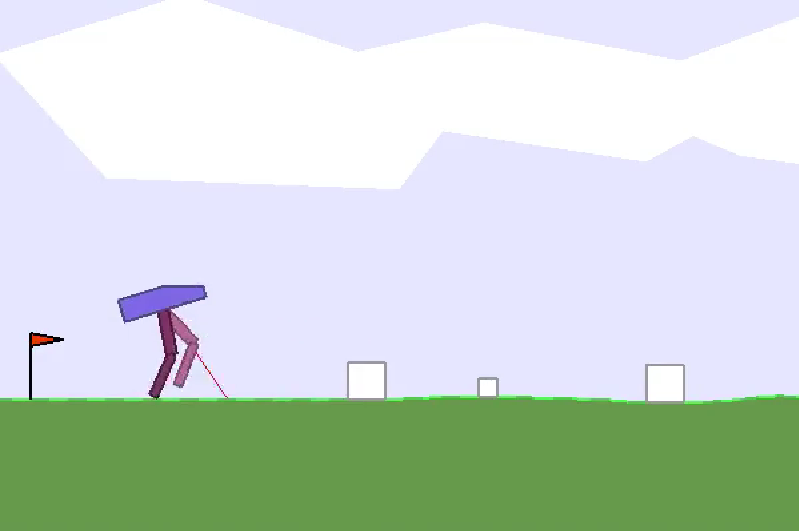
\includegraphics[width=0.9\linewidth]{figures/bipedal/hardcore.png}
		\caption{Bipedal-Walker-Hardcore-v3 Snapshot}
		\label{fig:bipedal_walker_hardcore}
	\end{subfigure}
	\caption{Bipedal Walkers Snapshots}
	\label{fig:bipedal_walkers}
\end{figure}
Locomotion of the Bipedal Walker is difficult control problem due to following reasons. \\
\begin{itemize}
	\item \textbf{Nonlinearity}: The dynamics is nonlinear, unstable and multimodal. Dynamical behavior of robot changes for different situations like ground contact, single leg contact and double leg concact. 
	\item \textbf{Uncertainity}: The terrain where robot walks may vary. Designing a controller for all types of terrain is difficult.
	\item \textbf{Partially Observability}: The robot observes ahead of it with lidar measurements and cannot observe behind. 
\end{itemize}
These difficulties make hard to implement analytical methods for control task. RL approach is better to tackle first 2 one. For partial observability problem, more elegant solution is required. This is done by creating a belief state from past observations to inform agent. Agent uses its belief state and observations to choose how to act. However, relying on observations is also possible. \\
\subsection{Deep Learning Library: PyTorch}
\label{dl_pytorch}
PyTorch is an open source library developed by Facebook's AI Research lab (FAIR) \cite{paszke_pytorch_2019}. It is based on Torch library \cite{collobert_torch7_2011} and has Python and C++ interface. It is an automatic differentation library with accelerated math operations backed by graphical processing units (GPUs). This is what a deep learning library requires. And the clean pythonic syntax made it most famous deep learning tool among researches. 
